\documentclass{article}%
\usepackage[T1]{fontenc}%
\usepackage[utf8]{inputenc}%
\usepackage{lmodern}%
\usepackage{textcomp}%
\usepackage{lastpage}%
\usepackage[head=40pt,margin=0.5in,bottom=0.6in]{geometry}%
\usepackage{graphicx}%
%
\title{\textbf{Instituto Prensa y Sociedad denunció censura de medios digitales en el país}}%
\author{El Nacional Web}%
\date{01/10/2018}%
%
\begin{document}%
\normalsize%
\maketitle%
\textbf{URL: }%
http://www.el{-}nacional.com/noticias/politica/instituto{-}prensa{-}sociedad{-}denuncio{-}censura{-}medios{-}digitales{-}pais\_253922\newline%
%
\textbf{Periodico: }%
EN, %
ID: %
253922, %
Seccion: %
Política\newline%
%
\textbf{Palabras Claves: }%
Libertad de expresión, Sociedad\newline%
%
\textbf{Derecho: }%
1.7, %
Otros Derechos: %
, %
Sub Derechos: %
\newline%
%
\textbf{EP: }%
SI\newline%
\newline%
%
\textbf{\textit{Mediante una investigación, el instituto indicó que varios medios un bloqueo casi total en los servicios de telecomunicaciones de Cantv y Movilnet}}%
\newline%
\newline%
%
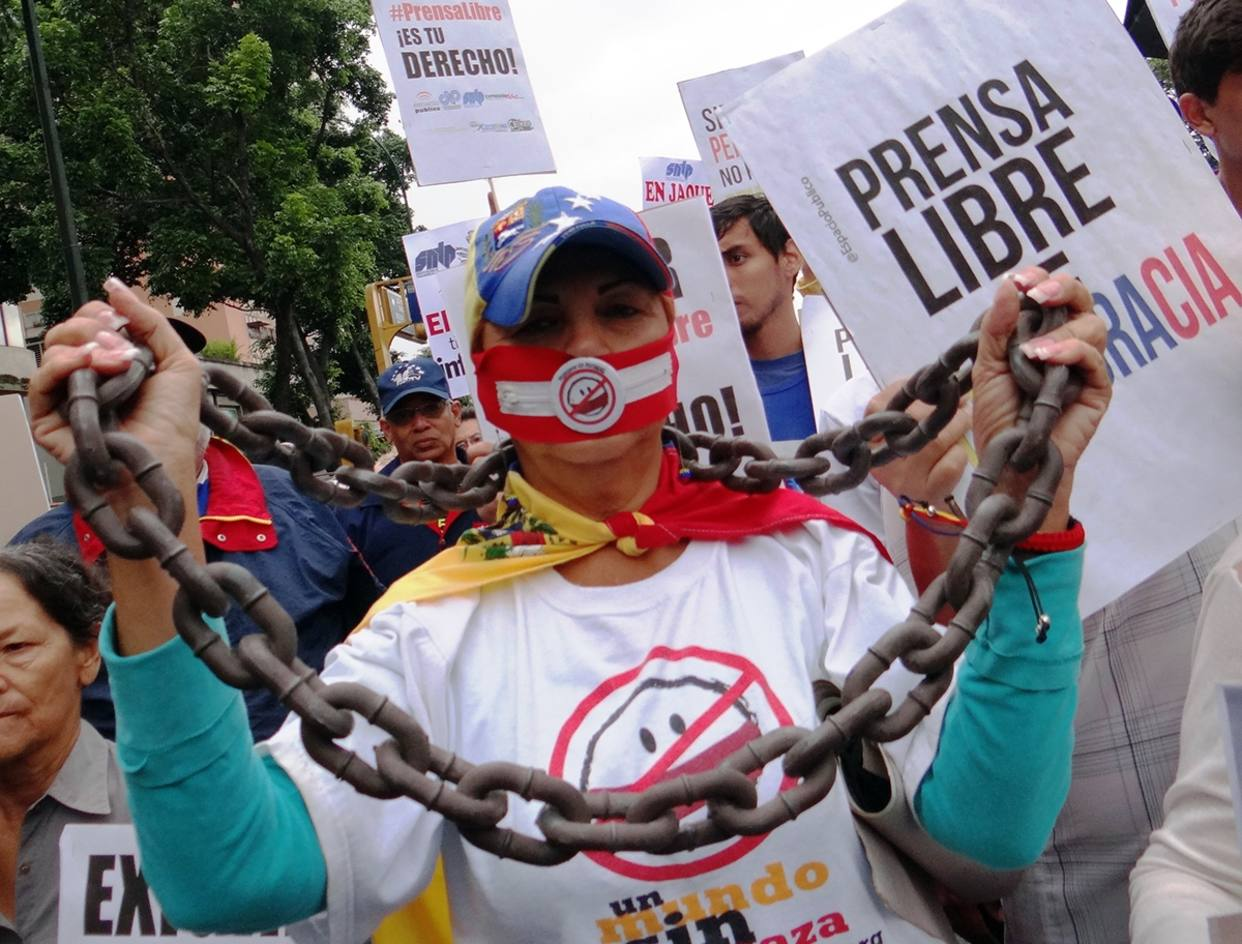
\includegraphics[width=300px]{113.jpg}%
\newline%
%
Una investigación sobre el bloqueo de páginas web~realizada por el Instituto Prensa y Sociedad de Venezuela (IPYS Venezuela) informó sobre~la existencia de~censura digital de portales informativos en el país.%
\newline%
%
Mediante una investigación, el instituto indicó que medios como~El Pitazo~y~NTN24~presentaron un bloqueo casi total en los servicios de telecomunicaciones de Cantv y Movilnet. Añadió que 53 portales siguen siendo considerados sensibles para las teleoperadoras, que han implementado tres modalidades de bloqueo, así lo informó~El Pitazo.%
\newline%
%
“Estas restricciones para acceder a las páginas monitoreadas –que incluyeron medios de comunicación y portales de información hípica y de cotizaciones del dólar paralelo– incumplen principios constitucionales y estándares internacionales sobre libertad de expresión y derecho a la información. El silencio impera en los principales actores estatales y privados encargados de administrar el acceso a los sitios web”, explicó~el estudio.%
\newline%
%
La organización no gubernamental indicó que el tipo de bloqueo a través del dominio de la página web, conocido como Bloqueo por DNS, es el obstáculo identificado más común.%
\newline%
%
Con información de~El Pitazo%
\newline%
%
\end{document}